\renewenvironment{longtable}{\rowcolors{2}{LightGray}{white}\oldlongtable} {\endoldlongtable}
\chapter{STM32及其编程简介}

\section{STM32是什么}
STM32是指意法半导体(STMicroelectronics)制造的一系列32位ARM架构单片机,这些单片机依据它们使用的核心不同,分为许多系列,例如本文档主要介绍的F1系列采用的是Cortex-M3内核 \footnote{https://en.wikipedia.org/wiki/STM32}。
作为单片机,STM32不仅包含了CPU核,还集成了Flash程序存储器、sRAM内存,以及诸如GPIO控制器的丰富外设,构成了一个片上系统(
\ac{SoC}
)。此外,STM32F1系列单片机的时钟频率可以高达72MHz,远超Arduino UNO的时钟频率,因此可以实现一些复杂的、繁重的控制任务,以及一些常用的算法。
\par 
本文档主要介绍的是STM32F103C8单片机,其中,这个命名包含的信息有:
\begin{itemize}
	\item STM32 - 表示ST生产的32位单片机
	\item F103 - 该单片机的系列
	\item C - 引脚数为48个
	\item 8 - Flash大小为64KiB\footnote{1 KiB = 1024 Bytes}
\end{itemize}
此外,它的内存容量为20KiB,是一款“中密度”单片机产品。
\par 
关于STM32F103C8的更详细的数据可以从它的Datasheet\footnote{https://www.st.com/resource/en/datasheet/stm32f103c8.pdf}中查到,这里不再继续对其进行介绍。

\section{STM32程序怎么写}
虽然我们认为这篇文档的读者以及掌握了基本的C语言程序设计,但是,在一个高度抽象的计算机上编程,与这里为单片机编程有着相当大的区别,所以,我们有必要从本质出发认识STM32程序的设计方法。
\subsection{程序的本质是什么}
程序的本质,当然是计算,毕竟程序是为“计算机”设计的。计算,可以认为是程序唯一的本质,CPU的所有行为不过是从存储介质中取得运算数,按程序对其计算,再将结果写入规定的存储介质中。可是这样,单片机是如何完成各种强大的控制功能的呢?这些功能,实际上是通过逻辑电路来实现的,CPU将控制这些逻辑电路的参数写入规定好的寄存器中,就可以告诉相应的逻辑电路该产生什么行为,除非遭遇了宇宙射线什么的,否则这些逻辑器件总是会乖乖听话。这就是单片机控制功能的来源。
\par 
不如举个例子,查阅STM32的参考手册\footnote{https://www.st.com/resource/en/reference\_manual/cd00171190.pdf}(\ac{RM}),可以知道GPIO这个外设有一个寄存器叫做“ODR (Port output data register)”,可以控制GPIO的输出电平,这个寄存器每个二进制位的意义如下图:
\par 
\begin{figure}[h]
	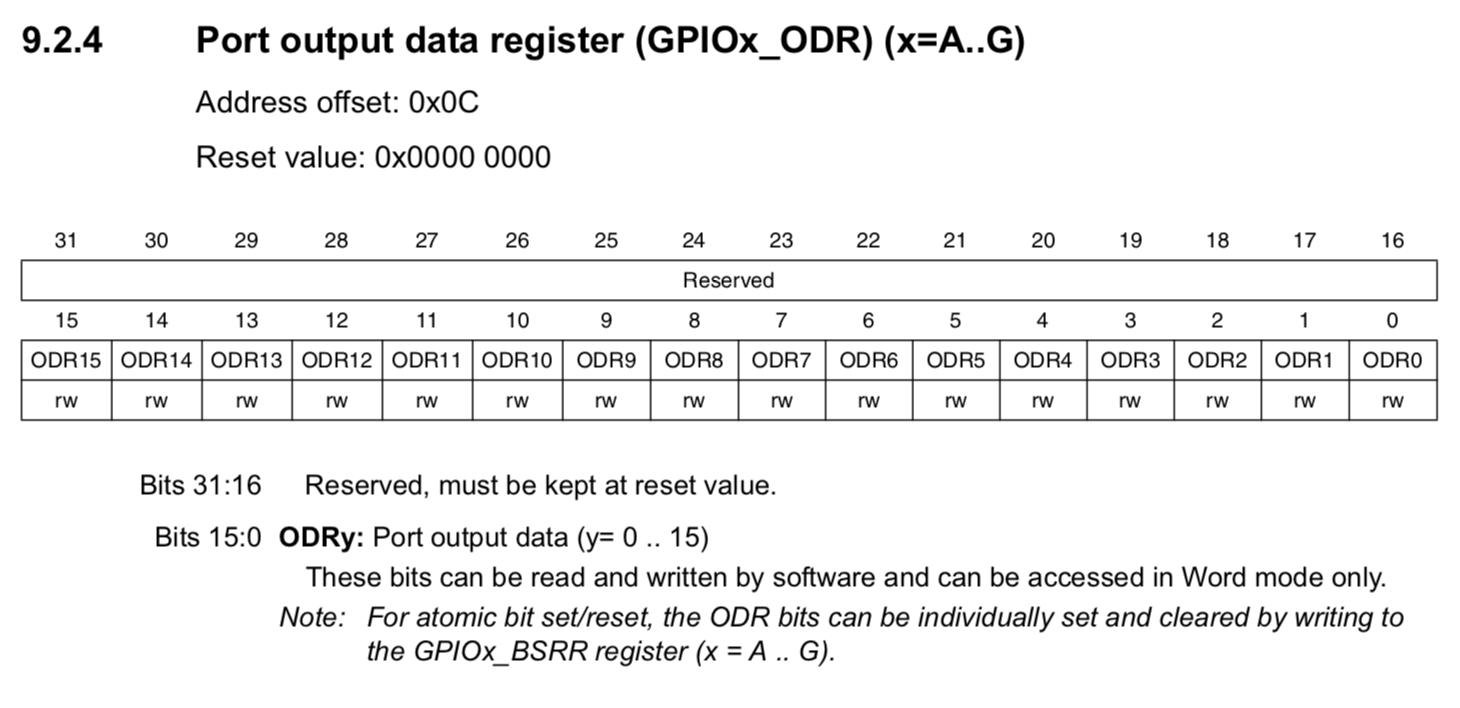
\includegraphics[width=\textwidth]{images/content/ODR.png}
	\captionof{figure}{ODR寄存器}
	\label{odrReg}
\end{figure}
\par 
假设GPIOA已经正确初始化,那么只要我们向GPIOA的ODR寄存器写入0x01,就可以控制PA0引脚输出高电平。为此,我们的程序可能长得像下面这样:
\par 
\begin{lstlisting}[language=bash, style=customStyleC, caption=控制PA0输出高电平]
GPIOA->ODR = 0x01;
\end{lstlisting}
\par 
实际上,完成这个操作的确这么简单,这一行程序的功能也没有超出“计算”的范围,因为它就是向一个指定的位置写入了一个预先算好的数据。
\par 
所以我们说,程序的本质是计算。

\subsection{我对象在哪儿}
在C语言中,一切对象皆是地址。
\par 
上面的代码中,并没有明显地表现出我们要操作的对象,GPIOA的ODR寄存器在哪里,事实上,仔细看看图\ref{odrReg},可以知道ODR寄存器的相对地址偏移(address offset)为0x0C,也就是说,在GPIOA的基地址上加上0x0C,就是GPIOA的ODR寄存器的绝对地址。有了地址,我们就可以对为所欲为了。再次查阅\acs{RM},知道GPIOA的基地址为0x40010800,所以控制PA0输出高电平还可以写成下面的形式:
\par 
\begin{lstlisting}[language=bash, style=customStyleC, caption=控制PA0输出高电平]
*(uint32_t*)(0x40010800 + 0x0C) = (uint32_t)0x01;
\end{lstlisting}
\par 
这行代码首先将地址0x40010800 + 0x0C转换为一个指向32位无符号整形数的指针,然后对其解引用,并写入0x01这个值,其功能与上一节中的代码完全一样。并且,只要单片机的初始化工作已经完成,这一行代码无需引入外部头文件即可编译通过。
\par 
当然,这样写代码还不如直接写汇编,所以我们要充分利用C语言的抽象性,利用结构体对外设进行建模。同样以GPIO这个外设为例,查阅\acs{RM}知道它的寄存器有下面这几个:
\begin{center}
	\begin{longtable}[l]{| p{30mm} | p{30mm} | p{80mm} |}
		\caption{GPIO寄存器}\\
		\hline 
		\rowcolor{Gray}
		\textbf{寄存器名称} & \textbf{地址偏移} & \textbf{简要描述} \\
		\hline
		\endfirsthead
		
		\hline 
		\rowcolor{Gray}
		\textbf{寄存器名称} & \textbf{地址偏移} & \textbf{简要描述} \\
		\hline
		\endhead
		
		CRL & 0x00 & 控制寄存器,控制0~7引脚 \\
		CRH & 0x04 & 控制寄存器,控制8~15引脚 \\
		IDR & 0x08 & 引脚输入寄存器 \\
		ODR & 0x0C & 引脚输出寄存器 \\
		BSRR & 0x10 & 引脚置位(置1)寄存器 \\
		BRR & 0x14 & 引脚复位(清0)寄存器 \\
		LCKR & 0x18 & 引脚锁存寄存器 \\
		
		\hline
	\end{longtable}
\end{center}
\par 
由于STM32是32位的单片机,因此其中的寄存器大多是32位的,即每一个寄存器占据的字节数是0x04,这与上表中的地址偏移之间的差值是一致的,从而可以发现这些寄存器的地址是连续分布的。这样,我们可以写出下面的结构体对GPIO的这几个寄存器进行抽象:
\par 
\begin{lstlisting}[language=bash, style=customStyleC, caption=GPIO结构体, label=periphStruct]
typedef struct GPIO_TypeDef {
	volatile uint32_t CRL;
	volatile uint32_t CRH;
	volatile uint32_t IDR;
	volatile uint32_t ODR;
	volatile uint32_t BSRR;
	volatile uint32_t BRR;
	volatile uint32_t LCKR;
} GPIO_TypeDef;
\end{lstlisting}
\par 
需要注意的是,这个结构体中各个成员数据的相对位置不能改变,类型也必须是32位大小的整形(最好是无符号的,以免运算时发生莫名其妙的符号位扩展),也不能增减成员,只有这样,才能正确地抽象GPIO的这些寄存器,与相应的地址空间对应。成员声明前面的volatile表明编译器不得对这个成员做出优化,意思是编译出来的程序必须老老实实的按照地址读写数据,而不能偷懒将它临时拷贝到CPU的寄存器中,这是因为这些GPIO寄存器并不是只有CPU才能读写,而电路本身就会更改它们的值。
\par 
利用这个结构体,我们就可以把从0x40010800开始的一段地址空间解释为GPIOA这个具体的外设,并对它进行操作:
\par 
\begin{lstlisting}[language=bash, style=customStyleC, caption=GPIO结构体应用]
GPIO_TypeDef * GPIOA = (GPIO_TypeDef *)(0x40010800);
GPIOA->ODR = 0x01;
\end{lstlisting}
\par 
这实际上解释了上一节的程序到底将0x01这个数据写到哪里了这个问题。
\par 
再强调一遍,C语言里,一切对象皆是地址,这个概念在STM32编程中尤为重要。所以下面,我们来欣赏一下STM32的地址空间映射\footnote{截自STM32F103C8 Datasheet}。
\par 
\begin{figure}[!h]
	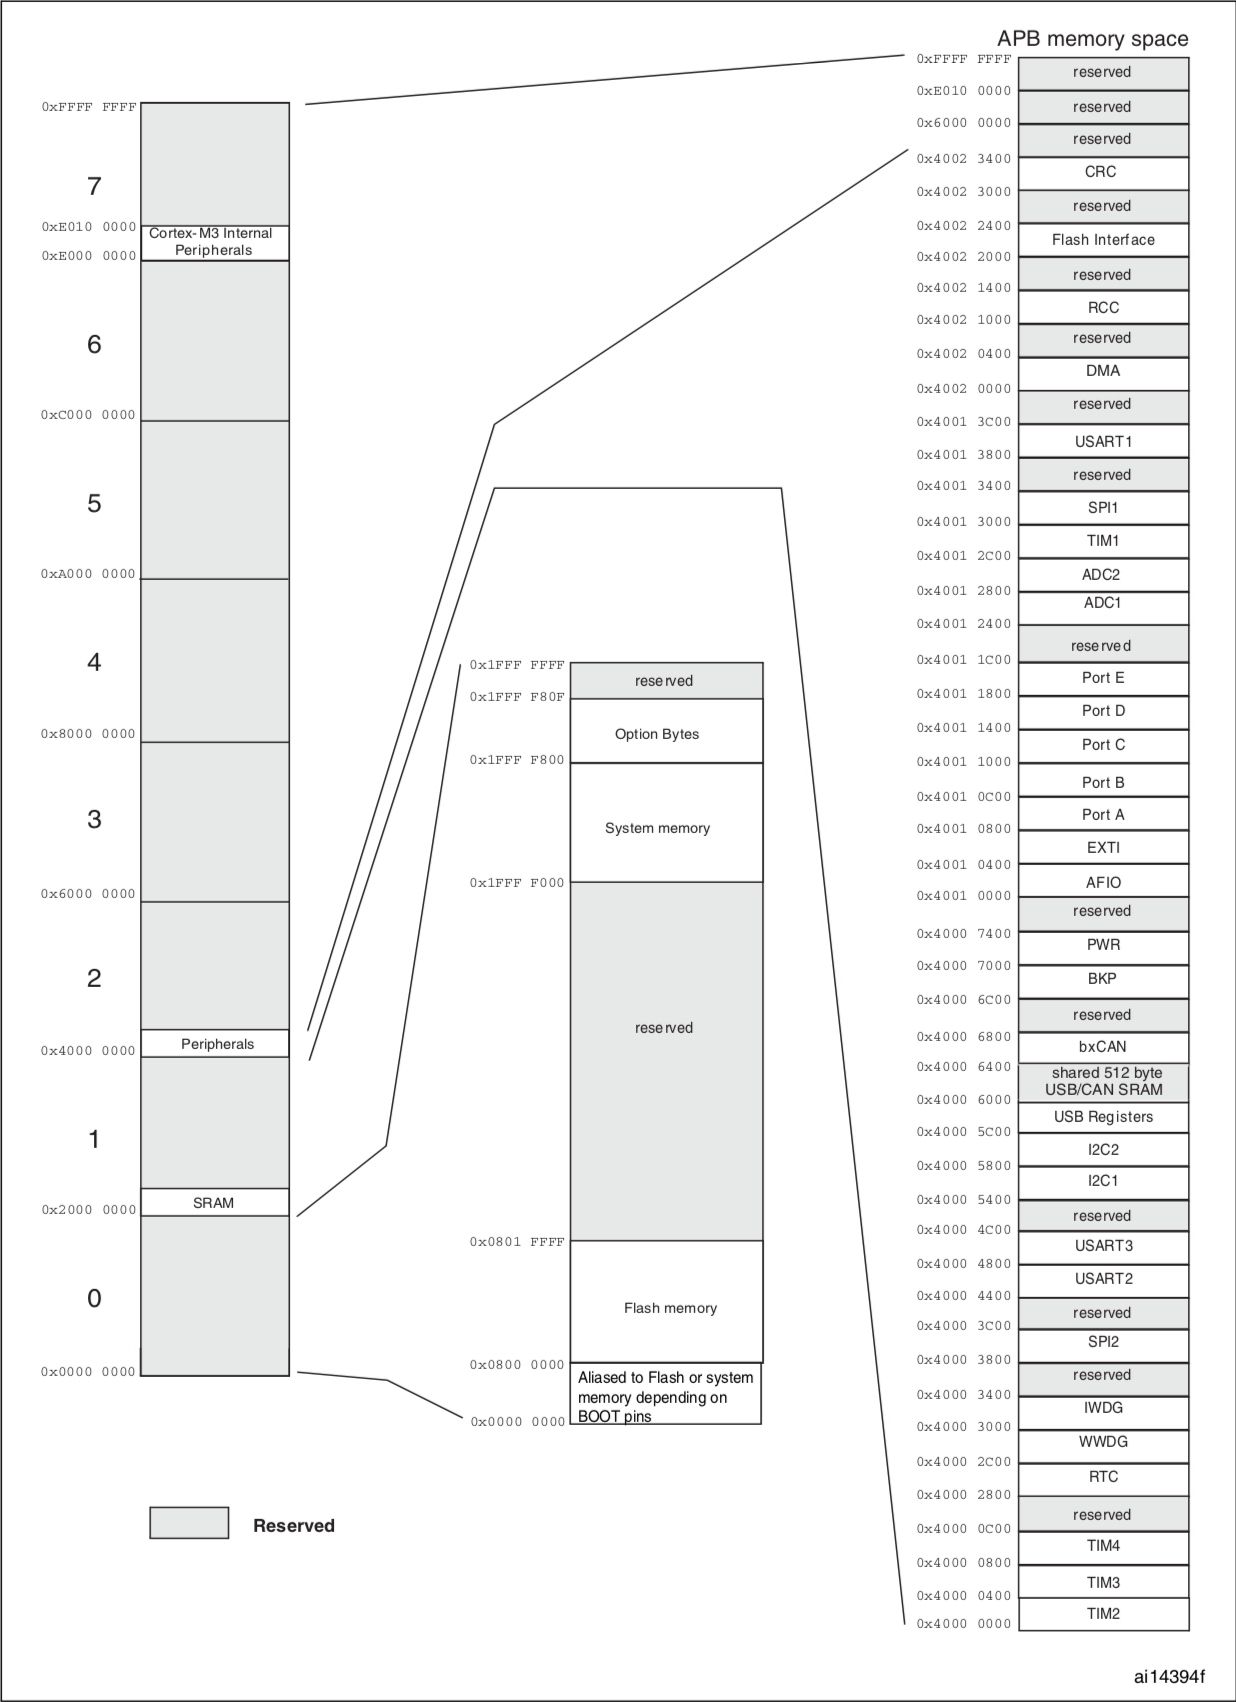
\includegraphics[width=\textwidth]{images/content/MemoryMap.png}
	\captionof{figure}{STM32地址空间映射图}
	\label{memoryMap}
\end{figure}
\par 
\subsection{STM32标准外设库}
我们不造轮子,但要知道轮子怎么造。
\par 
按照上一节的方法,对每一个外设逐一建模,再为每一个具体外设定义结构体变量,是一个相当庞大的工程,实现起来可能我们今年上半年就不用干别的了,而且就算实现了,用寄存器的方式操作外设难免会遇到许多玄学问题。因此,ST官方推出了标准外设库(Standard Peripherals Firmware Library),本文档采用的版本是3.5.0。目前,ST似乎把更多的精力转向了推广其\acs{HAL}(硬件抽象层)库,不过两者大同小异,而且功能都是完备的,所以不必太纠结使用哪个库,学会了其中一个就很容易触类旁通。
\par 
标准外设库用结构体、枚举类型及其宏定义的方式抽象出了STM32所有的外设资源,对于各种外设的基本操作,也提供了丰富的函数接口对其进行封装。使用标准外设库可以简化STM32程序的编写过程,而且其代码都是经过了专业的优化,具有很强的编译期查错能力,对于内存的占用也非常小,所以我们完全可以放心大胆地使用。
\par 
使用标准外设库,控制PA0输出高电平的语句就变得很直观:
\par
\begin{lstlisting}[language=bash, style=customStyleC, caption=控制PA0输出高电平]
GPIO_SetBits(GPIOA, GPIO_Pin_0);
\end{lstlisting}
\par
标准外设库的命名方式一般为“外设\_功能”的格式,所以对于代码补全非常友好,使用一个具有较强代码补全能力的编辑器(例如VS Code),多数情况下只需要打几个字母就能完成整行的输入。
\par 
既然官方已经为我们造好了这么方便的轮子,我们编写STM32的程序就可以处处应用标准外设库。本文档这一部分的介绍也将主要围绕着标准外设库的使用而展开。

\section{思考与练习}
\begin{enumerate}
	\item STM32F103C8的最高时钟频率是多少,如何理解这一数据?
	\item STM32F103C8的内存大小是多少?结合它的时钟频率,说明它适合执行怎么样的算法?举例说明不适合它执行的算法。当然,要考虑数据规模。
	\item 仿照代码清单\ref{periphStruct},参考\acs{RM},为外设SPI编写结构体进行抽象,并定义一个变量对应SPI1。完成后,对比标准外设库中的实现,想想为什么不一样(如果一样,那您就是巨佬)。
		\begin{lstlisting}[language=bash, style=customStyleC, caption=标准外设库中的SPI结构体]
		//其中的__IO是volatile的一个宏
		typedef struct
		{
			__IO uint16_t CR1;
			uint16_t  RESERVED0;
			__IO uint16_t CR2;
			uint16_t  RESERVED1;
			__IO uint16_t SR;
			uint16_t  RESERVED2;
			__IO uint16_t DR;
			uint16_t  RESERVED3;
			__IO uint16_t CRCPR;
			uint16_t  RESERVED4;
			__IO uint16_t RXCRCR;
			uint16_t  RESERVED5;
			__IO uint16_t TXCRCR;
			uint16_t  RESERVED6;
			__IO uint16_t I2SCFGR;
			uint16_t  RESERVED7;
			__IO uint16_t I2SPR;
			uint16_t  RESERVED8;  
		} SPI_TypeDef;
		\end{lstlisting}
	\item 标准外设库有什么好处?为什么不直接用寄存器编程?
	\item 简述操作STM32外设的本质。
\end{enumerate}











